\shorthandoff{"}
\chapter{Diskussion}
\label{ch:diskussion}

\section{Zusammenfassung der Forschungsergebnisse}
\label{ch:diskussion:zusammenfassung}
Im Rahmen der vorliegenden Master-Thesis wurde eine Fallstudie durchgeführt. Über diese wurden die Vorschläge eines unilateralen und eines bilateralen Empfehlungsansatzes bei der Besetzung offener Projektpositionen miteinander verglichen. Dabei konnte festgestellt werden, dass das bilaterale Vorschlagsverfahren bei vier der fünf evaluierten Projektpositionen eine höhere Zufriedenheit bei den Angestellten erzielen konnte. Bei einer Projektstelle sorgten dagegen der unilaterale Empfehlungsansatz für eine höhere Zufriedenheit.

Vergleichbar fielen auch die Ergebnisse auf Seiten der Projektmanager aus. Hier prognostizierten die Verantwortlichen für vier der fünf Projektpositionen eine höhere Arbeitsleistung von den vorgeschlagenen Mitarbeitern des bilateralen Empfehlungssystems. Einzig für die Stelle, bei welchen auch das bilaterale Vorschlagsverfahren eine geringere Zufriedenheit bei den Mitarbeitern erzielte, prognostizierten die Projektmanager für beide Empfehlungsansätze gleiche Arbeitsleistungen.

Außerdem wurde festgestellt, dass 17 Prozent der Mitarbeiter keine Kompetenzbewertung im Intranet der EXXETA AG vorgenommen hatten. Bei grafischer Darstellung von Präferenzen und beherrschten Fähigkeiten der Mitarbeiter konnte außerdem das lange (Ratten-)Schwanz beobachtet werden. Bezüglich der in den vordefinierten Projektpositionen benötigten Kompetenzen konnte festgestellt werden, dass die Anteile an Mitarbeitern, welche eine gesuchte Fähigkeit beherrschen und gleichzeitig präferieren und Angestellten, welche nicht über eine benötigte Kompetenz verfügen und diese dennoch präferieren, im Durchschnitt gleich groß sind. Darüber hinaus konnte beobachtet werden, dass knapp über 40 Prozent aller Mitarbeiter, welche eine gesuchte Fähigkeit beherrschen, deren Anwendung nicht als Präferenz angaben.

Abschließend wurde evaluiert, wie Mitarbeiter und Projektmanager mit möglicher Unterforderung bei der Projektarbeit umgehen. Diese Information ist gemäß der Theorie des \acp{PEFit} zur korrekten Berechnung der Kongruenz von Mitarbeiter und Projektposition notwendig. Im Rahmen der Befragung konnte hierbei festgestellt werden, dass sowohl Projektmanager als auch Mitarbeiter mehrheitlich eine Unterforderung vermeiden möchten.

\section{Interpretation der Forschungsergebnisse}
\label{ch:diskussion:interpretation}
In Kapitel \ref{ch:personEnvironmentFit:auswirkungenErhoehterAngebote} wurde beschrieben, dass ein P-E Misfit in drei möglichen Konsequenzen mit entsprechenden Gleichungen zur Berechnung resultieren kann. Im Rahmen der vorliegenden Master-Thesis wurde angenommen, dass sowohl Projektmitarbeiter als auch -manager eine Unterforderung bei der Besetzung offener Projektpositionen vermeiden möchten. Dementsprechend wurde Kurve B aus Abbildung \ref{fig:personEnvironmentFit:auswirkungenErhoehterAngebote:abb1} in Form der quadrierten Differenzberechnung implementiert. Die in Abbildung \ref{fig:ergebnisse:fallstudie:kurven:abb1} dargestellten Ergebnisse bestätigen auch diese Annahme sowohl aus Perspektive der Mitarbeiter als auch aus dem Blickwinkel der Projektverantwortlichen. 

Bei Implementierung der beiden Empfehlungsansätze wurde aufgrund der Erkenntnisse aus Kapitel \ref{ch:empfehlungssysteme} erwartet, dass der lange (Ratten-)Schwanz und der Kaltstart die Vorschlagserstellung beeinträchtigen könnten. Daher lag beiden Empfehlungsmethoden ein hybrider und graphenbasierter Ansatz zugrunde, welcher über die Einbeziehung von Fähigkeitsbewertungen und Teamzuordnungen beide Probleme löste. Dieses Vorgehen ist mit Blick auf die Ergebnisse in Abbildung \ref{fig:ergebnisse:analyse:abb1} als sinnvoll zu bewerten, da sowohl bei beherrschten als auch Präferierten Fähigkeiten ein langer (Ratten-)Schwanz erkennbar ist. Zusätzlich ist Kapitel \ref{ch:ergebnisse:analyse:intranetUndUmfrage} zu entnehmen, dass vier Mitarbeiter im Intranet keine einzige Fähigkeit bewertet hatten und diese ohne Einbeziehung der Teamzuordnungen folglich von einem Kaltstart betroffen wären.

Hinsichtlich der Kompetenzen konnte anhand von Abbildung \ref{fig:ergebnisse:analyse:abb3} außerdem beobachtet werden, dass die Mitarbeiter einen Großteil ihrer präferierten Fähigkeiten nicht beherrschen. Aus diesem Sachverhalt lässt sich schließen, dass die Angestellten bereit sind in Zukunft weitere Fähigkeiten zu erlernen und diese bei der Projektarbeit anzuwenden. Auf Unternehmensseite könnte dementsprechend der Einsatz weiterer formeller und informeller Weiterbildungsangebote evaluiert werden, bei welchen die Mitarbeiter nicht nur bestehende Kompetenzen vertiefen, sondern auch neue Fähigkeiten erwerben können.

Sowohl in Abbildung \ref{fig:ergebnisse:analyse:abb3} als auch Abbildung \ref{fig:ergebnisse:analyse:abb5} konnte beobachtet werden, dass das Beherrschen einer Fähigkeit keinen Rückschluss auf eine entsprechende Präferenz zulässt. Ein unilateraler Empfehlungsansatz würde dennoch sämtliche beherrschten Kompetenzen gleich behandeln. Somit ist davon auszugehen, dass die Angestellten bei Einsatz eines unilateralen Empfehlungssystems zumeist für Projektpositionen vorgeschlagen werden, deren gesuchte Fähigkeiten sie beherrschen. Hierbei ist die Wahrscheinlichkeit jedoch sehr groß, dass die Mitarbeiter einige diese Kompetenzen nicht anwenden möchten. Ein bilaterales System unterscheidet dagegen sowohl auf Ebene der beherrschten als auch der nicht beherrschten Fähigkeiten zwischen präferierten und nicht präferierten Kompetenzen. Da der Ansatz gewünschte Fähigkeiten stärker gewichtet, wird sich ein vorgeschlagener Mitarbeiter mit höherer Wahrscheinlichkeit die Anwendung der für die offene Projektposition benötigten Kompetenzen auch wünschen. Dementsprechend ist eine höhere Zufriedenheit und Motivation bei der Stellenbesetzung zu erwarten. Wie in Abbildung \ref{fig:diskussion:interpretation:abb1} zu erkennen, spiegelt sich diese auch in den Ergebnissen der Umfragen unter den Projektmitarbeitern und -managern der EXXETA AG wider.

\begin{figure}[h]
	\centering
	
	\subfloat[Zufriedenheit der Mitarbeiter mit den Beispielprojektpositionen]{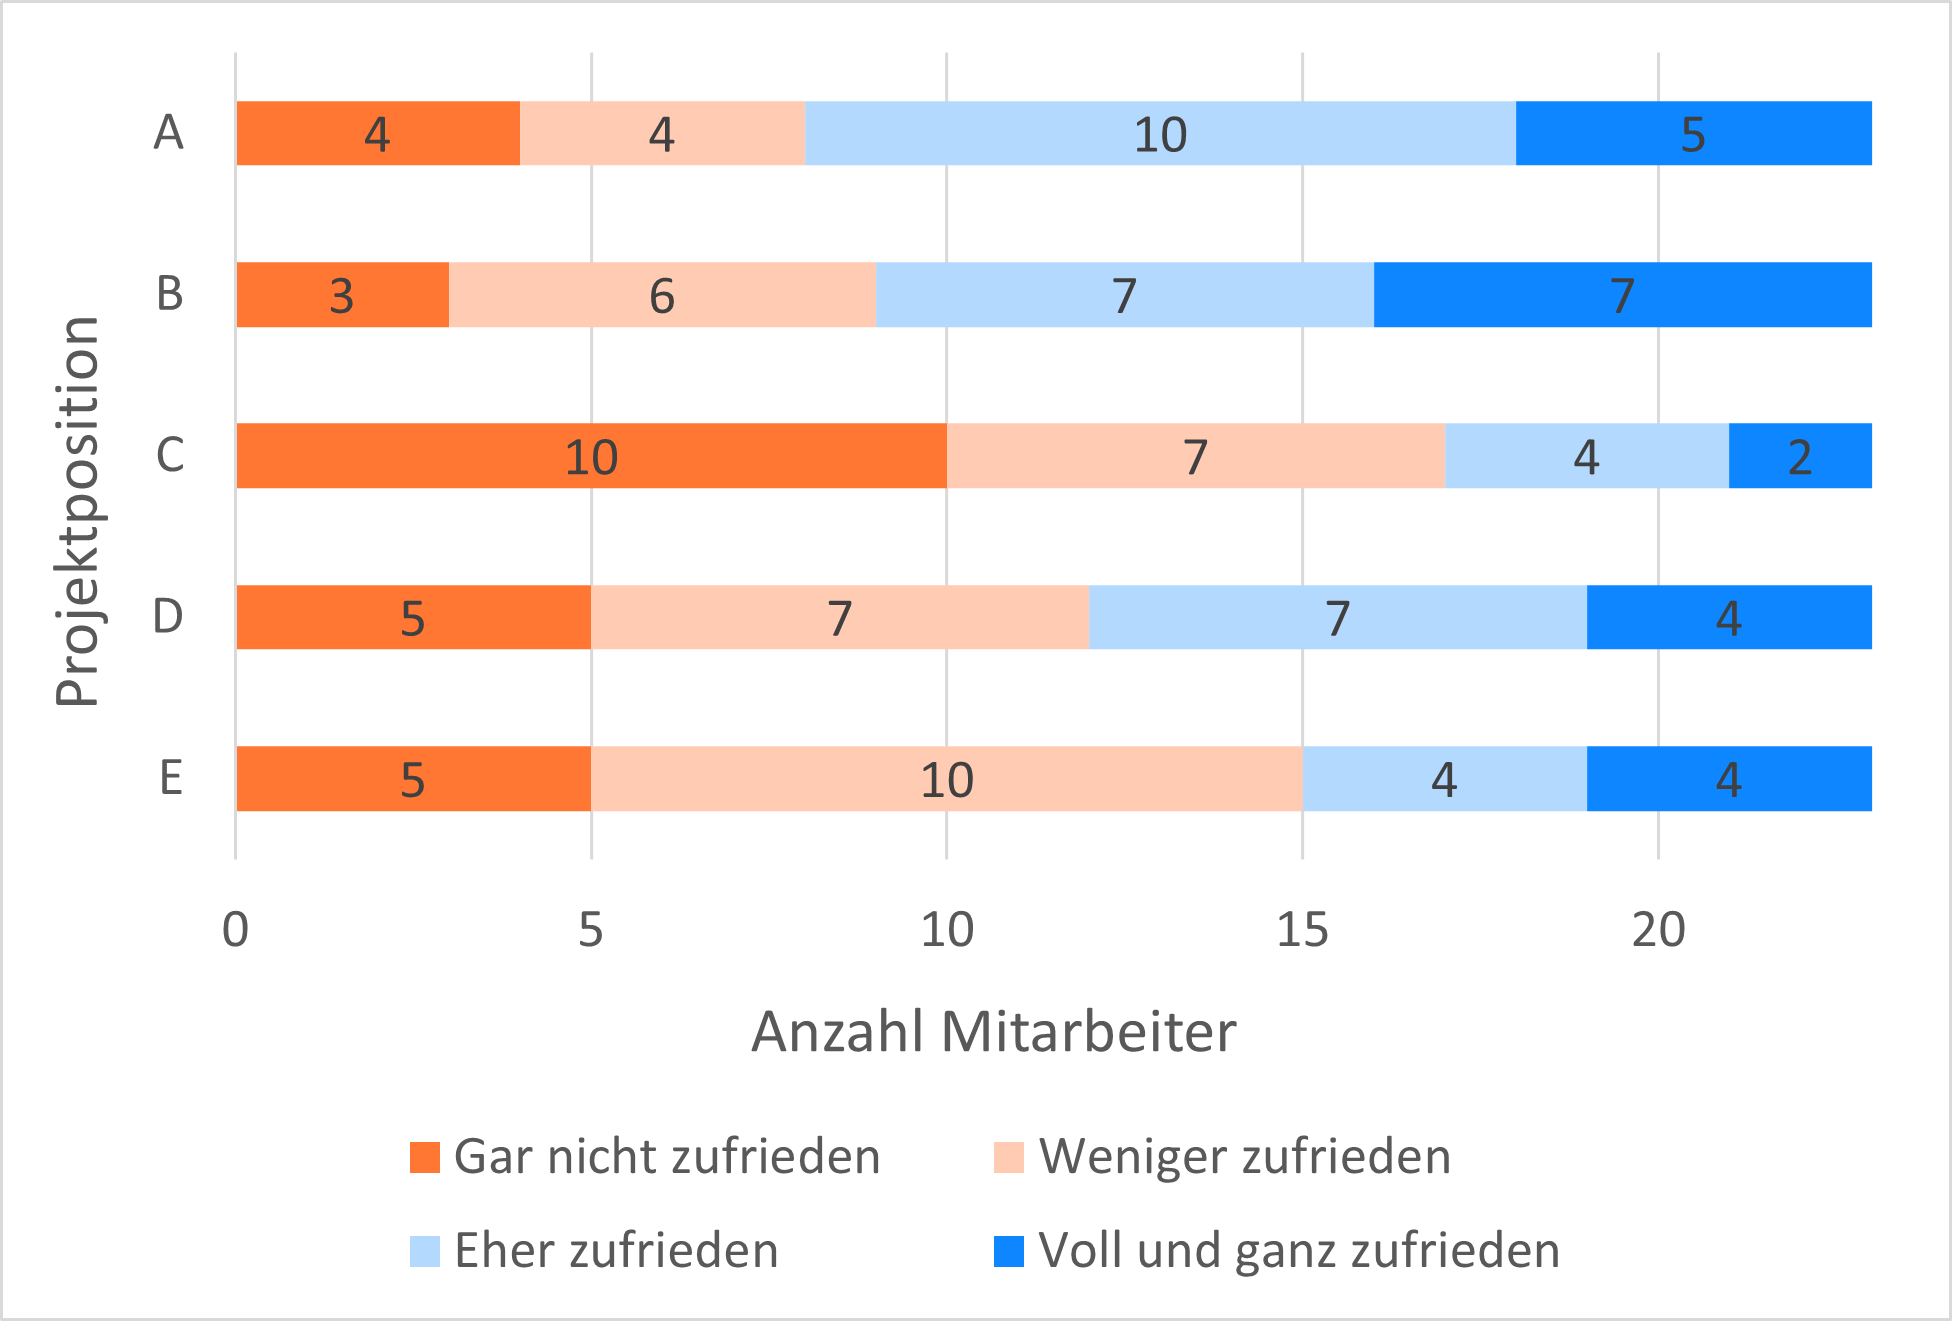
\includegraphics[width = 0.75\textwidth]{gfx/mitarbeiter-zufriedenheit-umfrage.png}}\\
	\subfloat[Ergebnisse Mitarbeiter]{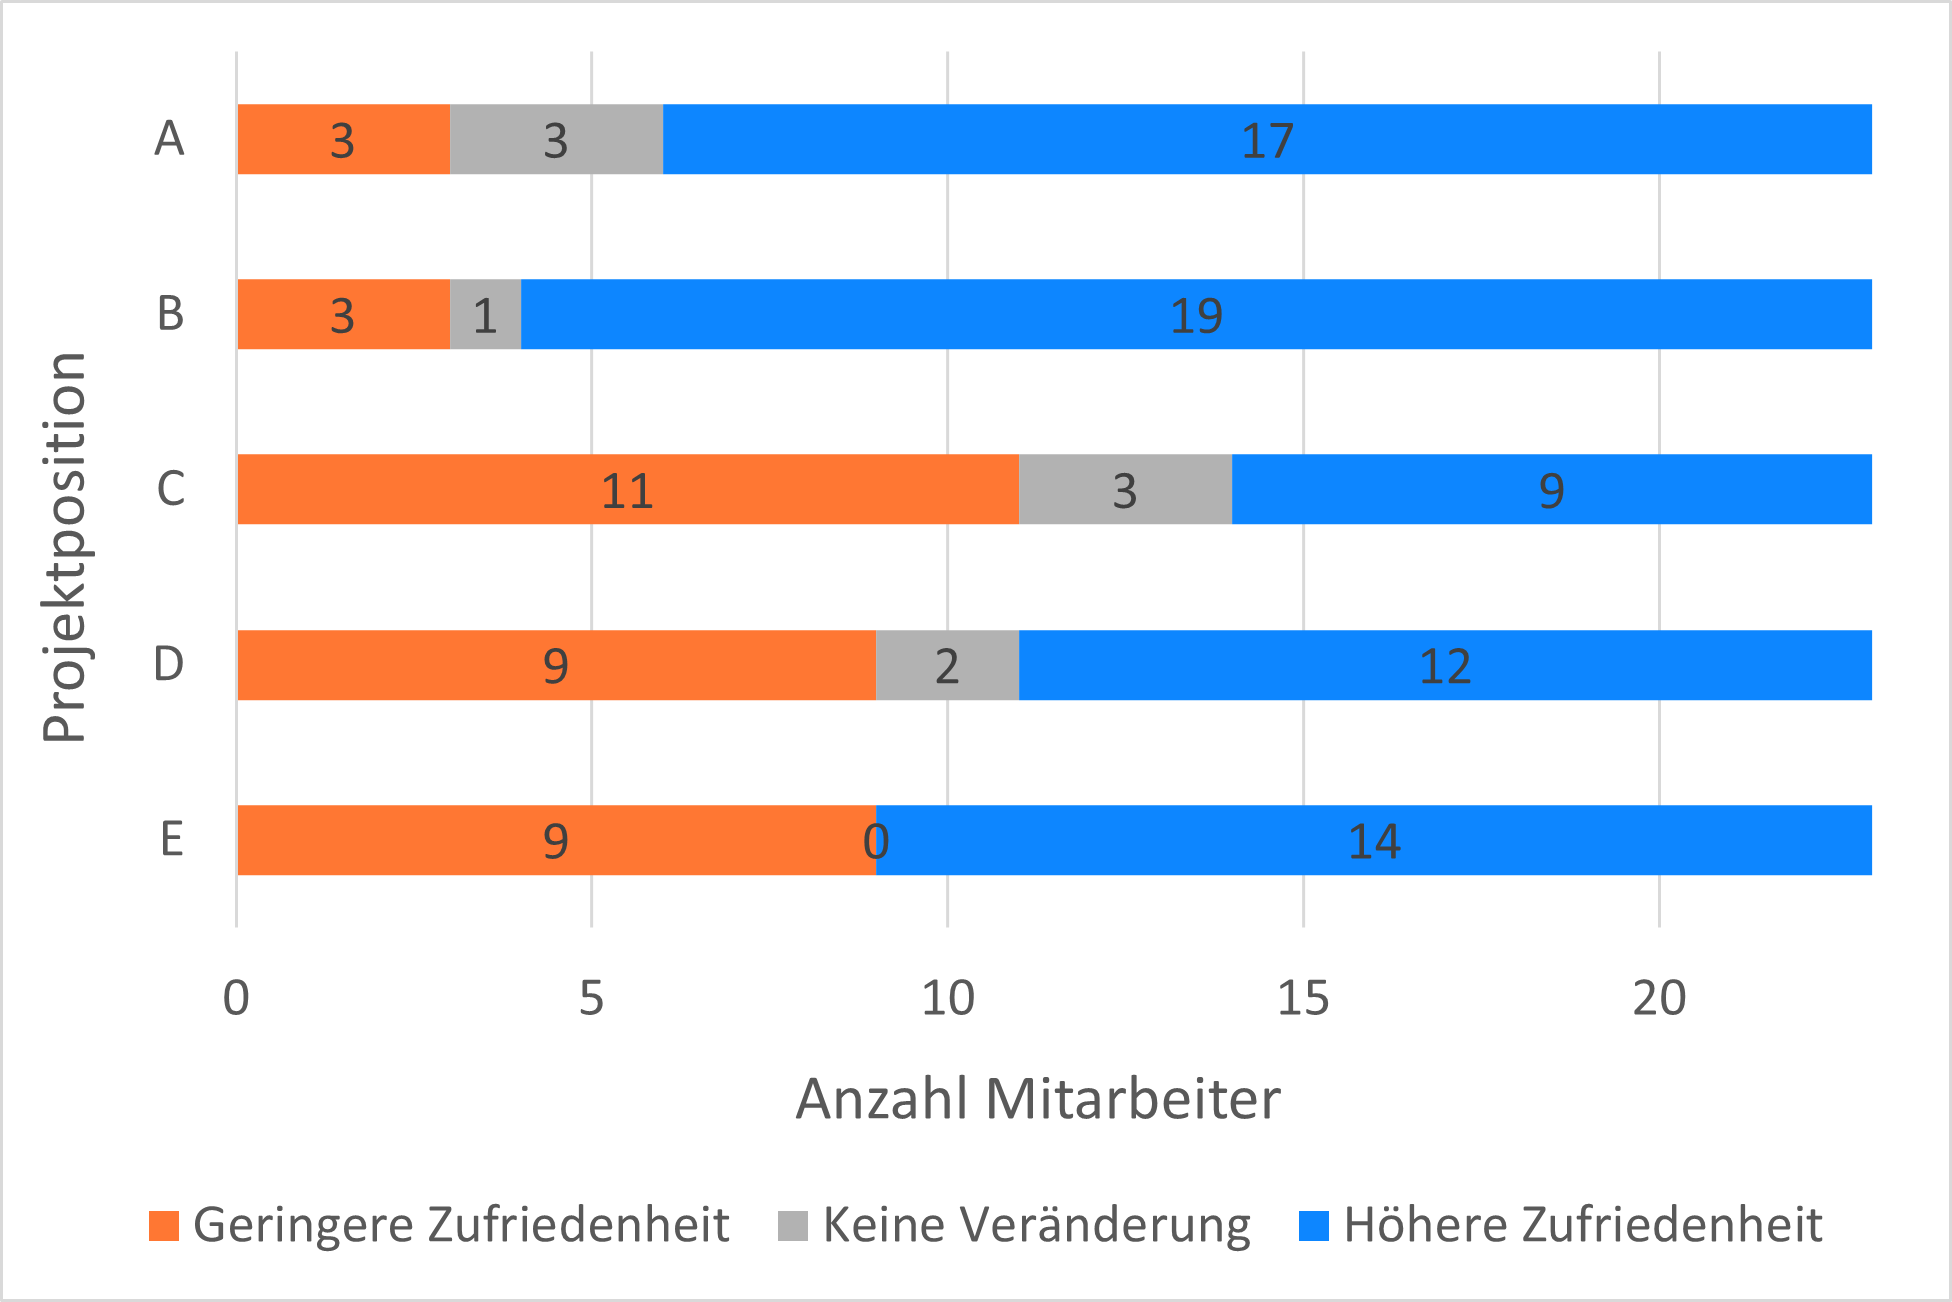
\includegraphics[width = 0.5\textwidth]{gfx/zufriedenheit-projekte.png}}
	\subfloat[Ergebnisse Projektmanager]{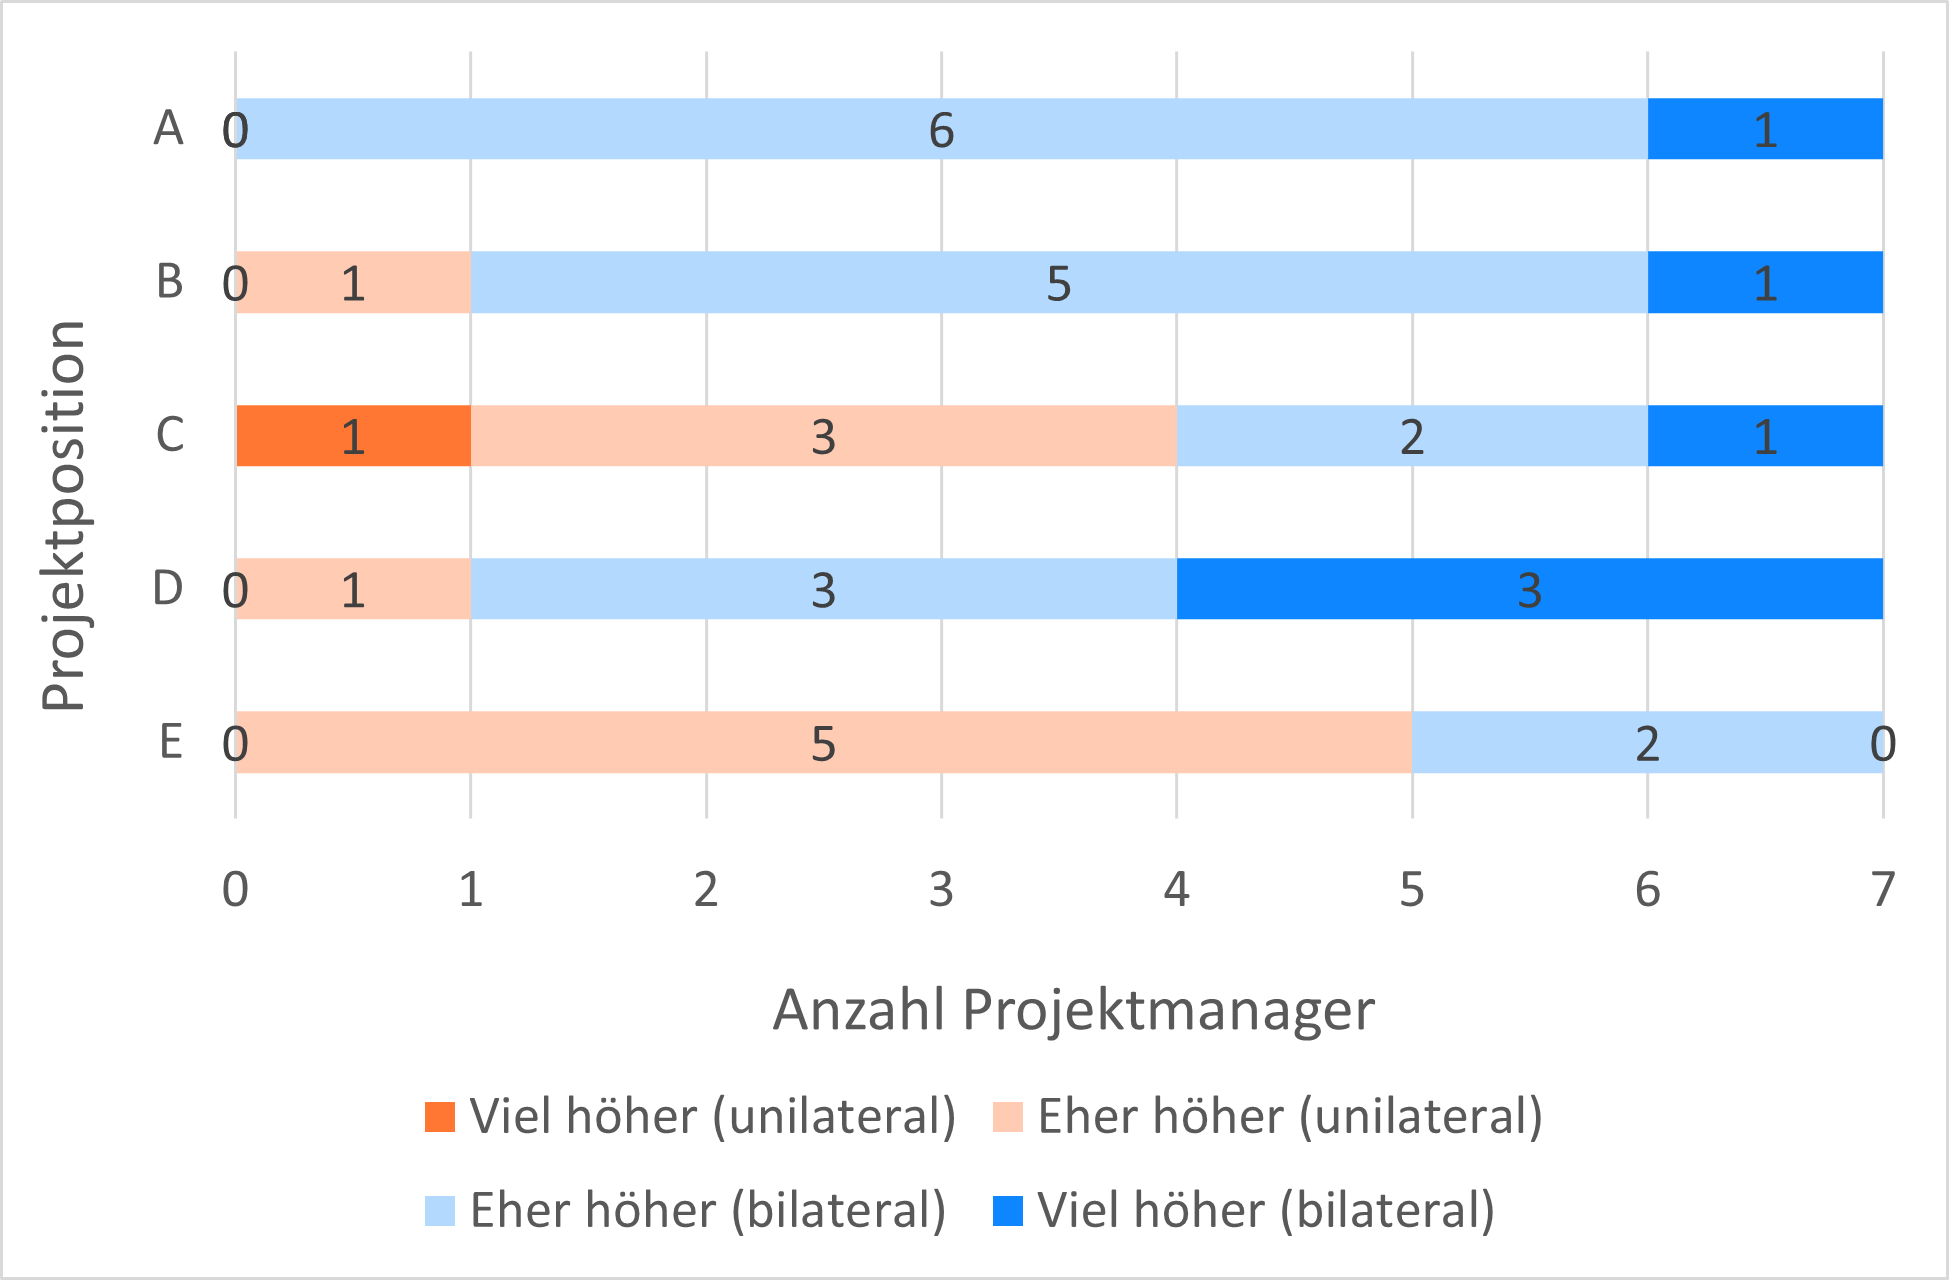
\includegraphics[width = 0.5\textwidth]{gfx/ergebnisse-projektmanager-arbeitsleistung.png}}
	
	\caption{Darstellung der Ergebnisse der Umfragen unter Mitarbeitern und Projektmanagern}
	\label{fig:diskussion:interpretation:abb1}
\end{figure}

An den Ergebnissen in Abbildung \ref{fig:diskussion:interpretation:abb1} ist zu erkennen, dass die Mitarbeiter durch das bilaterale Empfehlungssystem stärker zu deren Zufriedenheit positioniert werden, wenn diese eine hohe Zufriedenheit mit der Stelle prognostizieren. Dieser Sachverhalt ist insbesondere bei den Projektpositionen A und B zu beobachten. Mit diesen Stellen zeigen sich über die Hälfte der Mitarbeiter zufrieden. Gleichzeitig ordnet der bilaterale Empfehlungsansatz diese Angestellte in etwa dreiviertel der Fälle stärker zu deren Zufriedenheit an, als die unilaterale Methode. Zeigen sich dagegen weniger Mitarbeiter mit einer betrachteten Projektposition zufrieden, nimmt auch die Qualität des bilateralen Empfehlungsansatzes hinsichtlich der Mitarbeiterzufriedenheit ab. Besonders gut ist dieser Sachverhalt bei Projektposition C zu erkennen, mit welcher sich die Mitarbeiter mehrheitlich unzufrieden zeigen. Hier erzielt der bilaterale Empfehlungsansatz im Vergleich zur unilateralen Variante sogar Ergebnisse, welche zu einer geringeren Zufriedenheit der Mitarbeiter führen.

Ähnliche Ergebnisse können aus Abbildung \ref{fig:diskussion:interpretation:abb1} auch für die Perspektive der Projektmanager abgeleitet werden. Auch hier ist für die Projektpositionen A und B zu beobachten, dass die Verantwortlichen eine höhere Arbeitsleistung von den Vorschlägen des bilateralen Ansatzes erwarten, wenn sich die Mitarbeiter mit diesen Stellen zufrieden zeigen. Für die Projektpositionen C und E, mit welchen sich die Mitarbeiter mehrheitlich unzufrieden zeigen, erwarten die Projektmanager dementsprechend eine höhere Leistung von den Vorschlägen des unilateralen Empfehlungsansatzes.

Eine Ausnahme bildet Projektposition D in Abbildung \ref{fig:diskussion:interpretation:abb1}. Hier sorgen die Vorschläge des bilateralen Empfehlungsansatzes auf Seiten der Mitarbeiter für eine geringfügig gesteigerte Zufriedenheit und aus Perspektive der Projektmanager für eine viel höhere erwartete Arbeitsleistung. Die Erwartungen der Angestellten hinsichtlich ihrer Zufriedenheit mit der Stelle sind dagegen sehr ausgeglichen. Wie in Abbildung \ref{fig:diskussion:interpretation:abb2} zu erkennen, unterschieden sich die Vorschläge zu Projektposition D in der Umfrage unter den Projektmanagern in nur einer Person. Aus diesem Grund werden die Ergebnisse der Projektverantwortlichen als nicht repräsentativ betrachtet.

\begin{figure}[h]
	\centering
	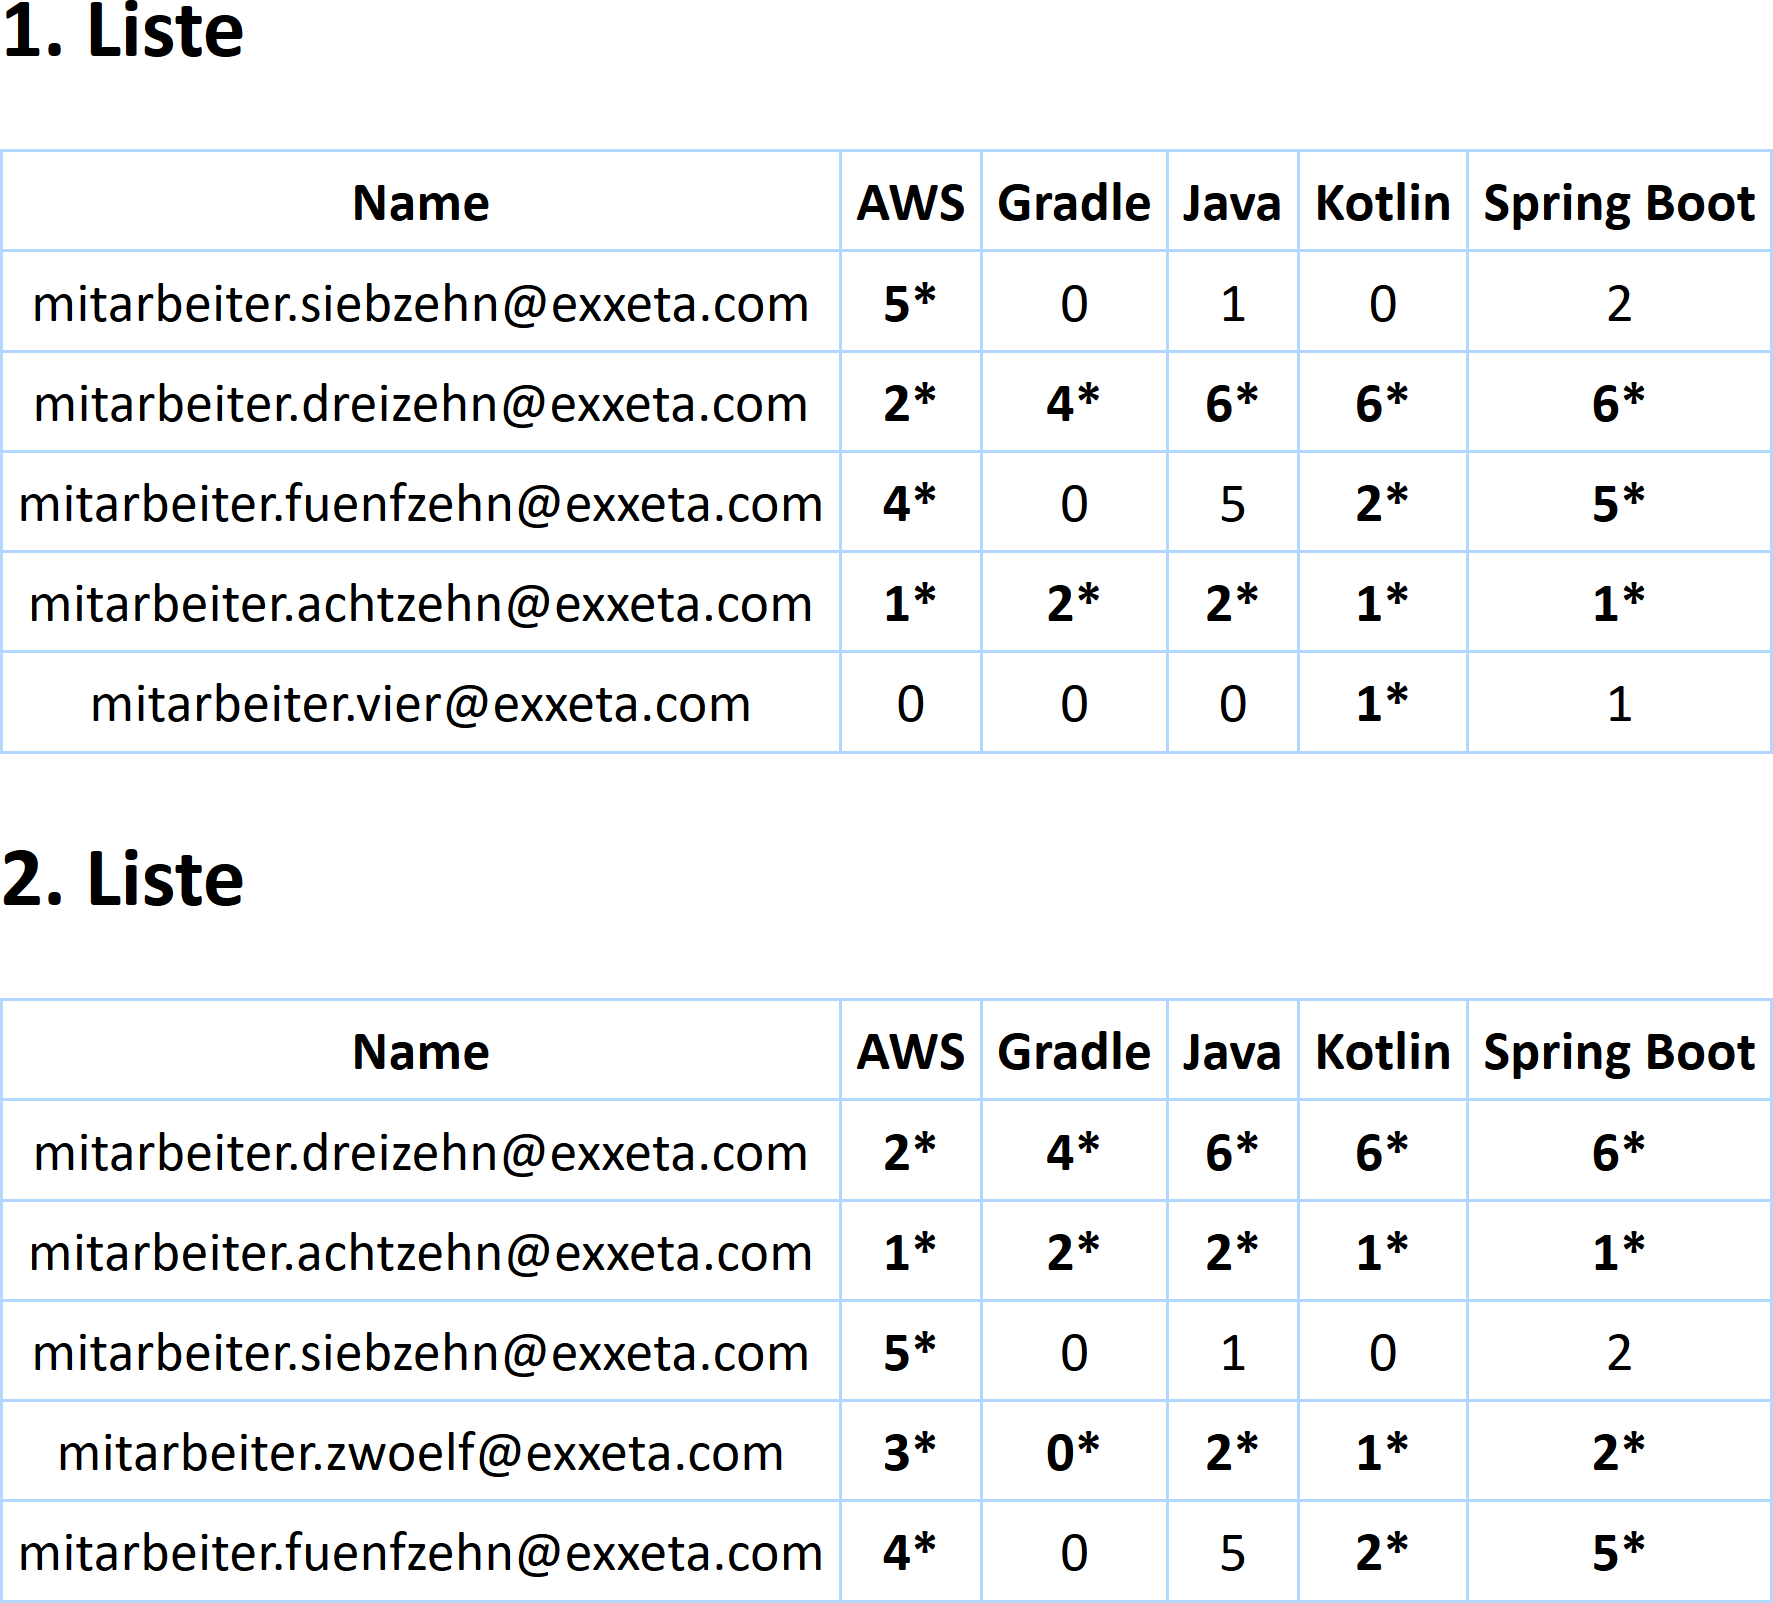
\includegraphics[width=0.65\textwidth]{gfx/projektposition-d.png}
	\caption{Mitarbeiter-Vorschläge für Projektposition D in der Umfrage unter den Projektmanagern (Pseudonymisiert)}
	\label{fig:diskussion:interpretation:abb2}
\end{figure}

Zur Beantwortung der Forschungsfrage ist damit festzustellen, dass die Anwendung eines bilateralen Empfehlungssystems bei der Besetzung offener Projektpositionen gleichzeitig die Zufriedenheit der Angestellten und die von den vorgeschlagenen Mitarbeitern erwartete Arbeitsleistung seitens der Projektmanager steigert. Diese Antwort gilt jedoch nur unter der Bedingung, dass sich die Mitarbeiter mehrheitlich zufrieden mit der betrachteten Projektposition zeigen.

Als Ursache für diese Einschränkung wird die Art der Erhebung der Präferenzen betrachtet. Die Mitarbeiter gaben im Rahmen der vorliegenden Master-Thesis ihre Wünsche über boolesche Werte an. Hierbei gewichtet das bilaterale Empfehlungssystem die Fähigkeiten der Angestellten höher, wenn sie diese präferieren. Es wurde jedoch nicht unterschieden, ob ein Angestellter einer nicht gewünschten Fähigkeit neutral gegenüber steht oder er diese nicht bei der Projektarbeit anwenden möchte. Einige der befragten Mitarbeiter, bei welchen es sich größtenteils um Backend-Entwickler handelt, könnten dementsprechend die für Projektposition C gesuchten kreativeren Kompetenzen nicht einsetzen wollen.

Aufgrund dieser Erkenntnisse wird für folgende Arbeiten empfohlen, den im Rahmen dieser Arbeit implementierten Empfehlungsansatz zu erweitern. Hierbei sollten die Präferenzen nicht über boolesche Werte, sondern über Abstufungen der Form "präferiert", "neutral", "nicht präferiert" erhoben werden. Ebenso wie die aktuelle Implementierung Mitarbeiter bei vorhandenem Wunsch höher positioniert, sollten Angestellte bei Angabe der negativen Präferenz niedriger einsortiert werden. Unter Betrachtung dieser Veränderungen sollte die Evaluation unter Mitarbeitern und Projektmanagern erneut durchgeführt und die Forschungsfrage entsprechend untersucht werden.

\section{Beschränkungen der Forschung}
\label{ch:diskussion:beschraenkungen}
- Sehr homogene Gruppe --> Alles Java-Entwickler (auch hier heterogen) --> Müsste überprüft werden, ob diese Ergebnisse auch für heterogene Gruppe zutreffen

\shorthandon{"}
